\chapter{Overview}
\label{c:overview}

%------------------------------------------------------------------------
\section{The Known Universe}

The information that \tao knows about can be divided into 5 categories: 
\begin{example}
  lattice   -- Machine layout and component strengths, and the beam orbit.
  data      -- Anything that can be measured. 
               For example: orbit data, dispersion data, etc.
  variables -- Anything that will typically be varied or used with the optimizer. 
               For example: quad strengths, etc.
  plotting  -- Display data and other stuff.
  global    -- Miscellaneous global parameters.
\end{example}
The \vn{lattice} and \vn{data} information are grouped into what is called a
\vn{universe}. The entire collection of \vn{lattices}, \vn{data},
\vn{variables}, \vn{plotting}, and \vn{global} information is called
the \vn{super_universe} and is the sum of everyhing \tao knows.

%------------------------------------------------------------------------
\section{Lattices}

A \vn{lattice} consists of a machine description (the strength and placement of elements)
along with the beam orbit through them. There are actually three types of lattices:
  \vspace*{-3ex}
  \begin{description}
  \item[Design Lattice] \Newline 
The \vn{design} lattice is the particular lattice that one wants the
actual physical machine to conform to. The \vn{design} lattice is fixed. Nothing is
alowed to vary in this lattice.
  \item[Model Lattice] \Newline
All \tao commands to vary lattice variables vary quantities in the
\vn{model} lattice. In particular, things like orbit correction
involve varying \vn{model} variables until the \vn{data} as calculated
from the \vn{model} match the \vn{data} as actually measured.
  \item[Base Lattice] \Newline
It is sometimes convenient to designate a reference lattice so that
changes in the \vn{model} from the reference point can be looked at.
This reference lattice is called the \vn{base}.
  \end{description}

The \vn{model}, \vn{design}, and \vn{base} lattices along with any
\vn{data} are bundled together to form what is called a
\vn{universe}. \tao can simultaneously handle multiple universes. Why
is this useful? It can be used, for example, to simulate both rings of
a collider machine. This can be convenient if there are, say, steering
elements in common and it is needed to simultaneously correct the
orbit in both rings. Another case is where orbits in a machine have
been measured under different conditions of, say, beam energy, and it
is desired to fit all the data simultaneously.

%------------------------------------------------------------------------
\section{Data}

Blocks of like data are associated with what are called \vn{d1_data}
structures and sets of \vn{d1_data} structures are collected into what
are called \vn{d2_data} structures. For example, a \vn{d1_data}
structure is typically associated with the horizontal orbit data and
another \vn{d1_data} structure is typically associated with the
vertical orbit data. These two structures can then be collected into a
\vn{d2_data} structure representing all orbit data. The \vn{d1_data}
and \vn{d2_data} structures are defined in the \tao initialization
file (cf.~Chapter~\ref{c:init}).  When issuing \tao commands, all the
data associated with a \vn{d2_data} structure is specified using the
\vn{d2_data} structure's \vn{name}.  The data associated with a
\vn{d1_data} structure is specified using the format
\vn{d2_name:d1_name}. For example, If a \vn{d2_data} structure has the
name ``\vn{orbit}'', and one of its \vn{d1_data} structures has the name
``\vn{x}'', then in \tao commands you refer to the data in this
\vn{d1_data} structure by the name ``\vn{orbit:x}''. Sometimes there is
only one \vn{d1_data} structure for a given \vn{d2_data} structure. In
this case the data can be referred to simply by using the
\vn{d2_data} structures's name.

Each data point (for example, the horizontal orbit at some
detector) has a number of quantities associated with it:
  \vspace*{-3ex}
  \begin{description}
  \item[Measured Data] \Newline 
The data as obtained from some measurement. This is what is used when running the optimizer.
When doing lattice design the measured \vn{data} corresponds to
a constraint (See chapter~\ref{c:opti} on optimization for more details).
  \item[Reference Data] \Newline
Reference data obtained from some reference measurement. For example,
a measurement before some variable is varied could be designated as
the \vn{reference}, and the data taken after the variation could be 
designated the \vn{measrued} data.
  \item[Model Data] \Newline
The data as calculated from the \vn{model} lattice.
  \item[Design Data] \Newline
The data as calculated from the \vn{design} lattice.
  \item[Base Data] \Newline
The data as calculated from the \vn{base} lattice.
  \end{description}

Use the \vn{show data} command to view information about any data.

\vfill
\break
%------------------------------------------------------------------------
\section{Variables}

Blocks of variables are associated with what is called a
\vn{v1_var} structure and each of these structures has a \vn{name}
with which to refer to them in \tao commands. A given variable may
control a single attribute of one element in a \vn{model} lattice
of a single universe or variables can be configured to simultaneously
control an element attribute across multiple universes. Any one variable 
cannot control more than one attribute of one element. However, a variable
may control an overlay or group element, which in turn controls numerous elements.

Each individual variable has a number of values associated with it:
  \vspace*{-3ex}
  \begin{description}
  \item[Measured Value] \Newline
The Value as obtained at the time of the \vn{data} measurement.
  \item[Reference Value] \Newline
The Value as obtained at the time of the \vn{reference} data  measurement.
  \item[Model Value] \Newline
The value as given in the \vn{model} lattice.
  \item[Design Value] \Newline
The value as given in the \vn{design} lattice.
  \item[Base Value] \Newline
The value as given in the \vn{base} lattice.
  \end{description}

Use the \vn{show var} command to view variable information

\vfill
\break
%------------------------------------------------------------------------
\section{Plotting}

\begin{figure}
  \centering
  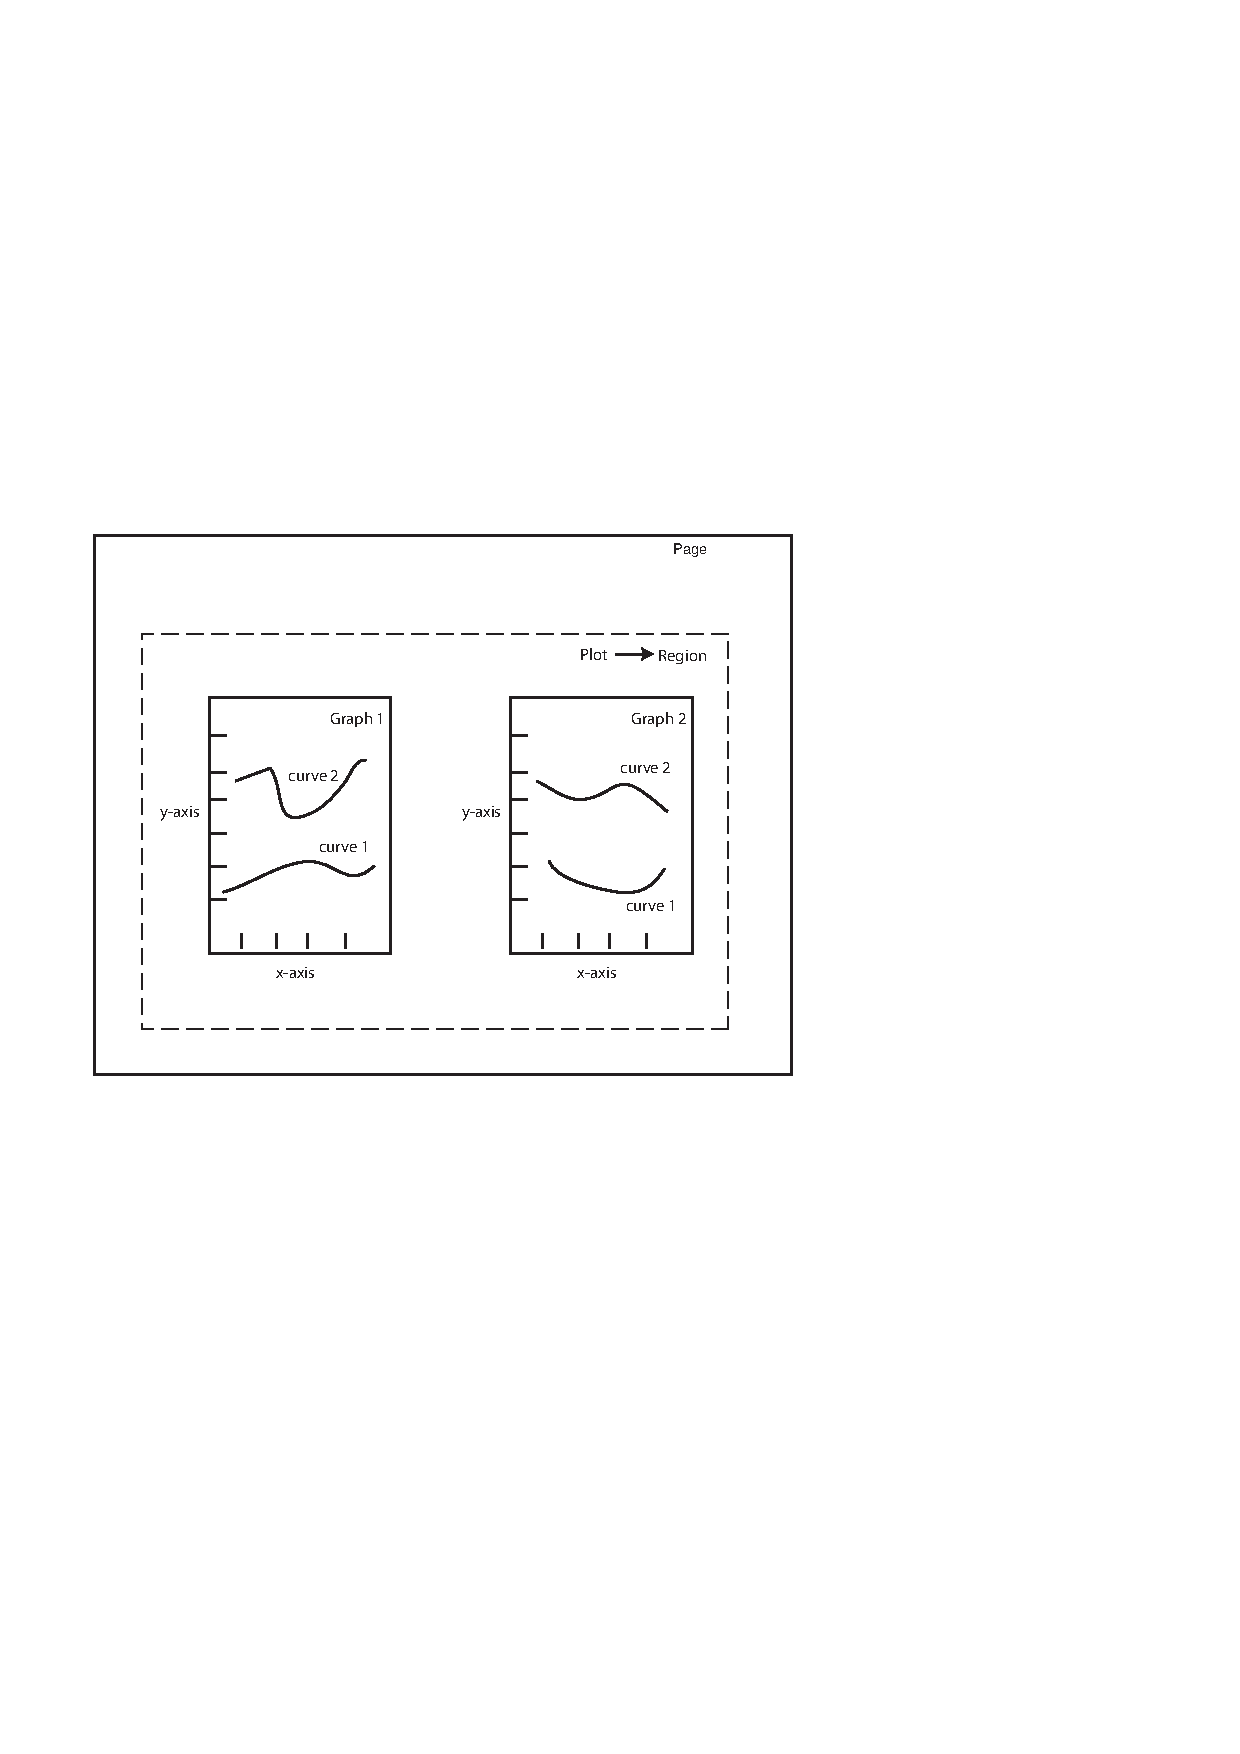
\includegraphics{plot.psfig}
  \caption{A plot has is a collection of graphs and a graph has a 
collection of curves. A plot becomes visible when it is associated
with some region on the page using the \vn{place} command. Note that
on the actual page the plot/region border is not visible.}
  \label{f:plot}
\end{figure}

Some definitions:
  \vspace*{-3ex}
\begin{description}
\item[Curve] \Newline
A \vn{curve} is a set of (x,y) points to be plotted.
\item[Graph] \Newline
A \vn{graph} consists of horizontal and vertical axes along with a set
of \vn{curve}s that are plotted within the graph. 
\item[Plot] \Newline
A \vn{plot} is essentially a collection of \vn{graphs}.
\item[Page] \Newline
The \vn{page} refers to the x--window where graphics are displayed or the 
corresponding printed graphics page.
\item[Region] \Newline
The \vn{page} is divided up into a number of rectangles called
\vn{regions}. \vn{Regions} may overlap.
\end{description}

The plot initialization file (cf.~Chapter~\ref{c:init}) defines a set
of \vn{template plots}. A \vn{template} defines what type of data is
to be plotted (orbit, coupling, etc.), how many \vn{graphs} there are,
what the scales are for the \vn{graph} axes, how the \vn{graph}s are
laid out, etc.  The plot initialization file also defines a set of
\vn{region}s within the \vn{page}. Any \vn{template plot} can be placed in any region.
 Using the \vn{place} command  
(see Chapter~\ref{c:command} for a full descriptions of all commands) one
can assign a particular \vn{template plot} to a particular region for plotting.
The relationship between \vn{region}, \vn{plot}, \vn{graph}, and
\vn{curve} is shown graphically in Figure~\ref{f:plot}.

Figures~\ref{f:plot_page1} and \ref{f:plot_page2} show examples of a
plot \vn{page}. Figure~\ref{f:plot_page1} was generated by defining
two regions called \vn{top} and \vn{bottom} in the plot initialization
file. The \vn{top} region was defined to cover the upper half of the
\vn{page} and the \vn{bottom} region was defined to cover the bottom
half. \vn{Template plots} were defined to plot phase and orbit data
from a defined set of detector elements in the lattice. Each
\vn{template plot} defined two graphs which in both cases where
assigned the names \vn{x} and \vn{y}. The orbit \vn{template plot} was
placed in the \vn{top} region and the phase \vn{template plot} was
placed in the \vn{bottom} region. The horizontal axis numbering is by
detector \vn{index}.  Displayed plots are referred to by the
\vn{region} name (\vn{top} and \vn{bottom} in this case). Individual
graphs are referred to using the nomenclature
\vn{region:graph}. Thus, in this example, the horizontal orbit graph
would be referred to as \vn{top:x}.  Using the \vn{plot} command one
can then specify \vn{who} is plotted. \vn{who} refers to
\vn{measured}, \vn{reference}, \vn{model}, \vn{base}, and/or
\vn{design} data.  Notice that the same \vn{template plot} can be
assigned to different \vn{regions} and the plots in different
\vn{regions} can have different scales for their axes or different
\vn{who}. In the example in Figure~\ref{f:plot_page1}, \vn{who} for the
\vn{top} plot is \vn{model} and for the \vn{bottom} plot it is
\vn{model-design}.

The \vn{use}, \vn{veto}, \vn{restore}, and \vn{clip} commands are used
to display or not to display individual data points. These are the
same commands that control what data is used in fitting the model to
the data in the optimization process (see Chapter~\ref{c:opti}). The
general rule is that data that is vetoed for display is also vetoed
for fitting. However, data that is off the vetical or horizontal scale may still
be used by the optimizer unless vetoed with the \vn{veto} or \vn{clip} command.
If there are data points off the vertical scale and are still used by the
optimizer then ``**Limited**'' will appear in the upper right-hand corner of the
graph.

The \vn{x-axis} and \vn{x-scale} commands are used to set the axis type and
scale for each graph. The axis type can be either \vn{index}, \vn{ele_index} 
or \vn{s} which
corresponds to the data index number, element index number and longitudinal 
poisition in the lattice
(from element 0) respectively.

Figure~\ref{f:plot_page2} shows another example of a plot \vn{page}.
In this case the \vn{page} was generated by again defining two
vertically stacked regions but in this case the regions have different
heights.  A \vn{template plot} with a single graph was placed in the
bottom most \vn{region}.  This \vn{graph} contains a \vn{key_table}.
A \vn{key_table} is used in conjunction with \vn{single mode} and is
explained in Chapter~\ref{c:single}. A \vn{template plot} containing
five \vn{graphs} was placed in the uppermost region. The uppermost
\vn{graph} of this \vn{template plot} contains a \vn{lat_layout} which
shows the placement of lattice elements.  What elements are displayed
in a \vn{lat_layout} and what shapes they are represented by is
specified in the initialization file. The horizontal scale is
longitudinal position (\vn{s}).  The remaining four graphs show
disperion and beta data from two different universes representing the
low energy and high energy transport in an energy recovery linac. The
individual data points here (hard to see in this example) have been
slaved to the \vn{lat_layout} and represent the beta and dispersion at
the edges of the displayed elements in the \vn{lat_layout}.


\begin{figure}
  \centering
  \includegraphics[width=5in]{plot_page1.psfig}
  \caption{Example of a plot page}
  \label{f:plot_page1}
\end{figure}

\begin{figure}
  \centering
  \includegraphics[width=5in]{plot_page2.psfig}
  \caption{Another example of a plot page.}
  \label{f:plot_page2}
\end{figure}

\vfill
\break
%------------------------------------------------------------------------
\section{Single Character Input}

Sometimes it is convenient to be able to vary variables using single
key strokes without having to type a carriage return.  With \tao this
is possible using what is called \vn{single mode}. This is distinct
from \vn{line mode} where commands to \tao are typed at the command
line with a carriage return signaling the end of the command. As
explained in the initialization chapter, \vn{single mode} uses a
special initialization file.

The \vn{single mode} initialization file associates variables with
certain keyboard keys so that when these keys are pressed the value of
the variable is varied. This association between variables and keys is
called a \vn{key table}.

%------------------------------------------------------------------------
\section{Tracking Types}

The are two types of tracking implemented in \tao: single particle
tracking and macroparticle tracking. Single particle tracking is just
that, the tracking of a single particle through the
lattice. Macroparticle tracking takes a beam distribution and tracks
the centroids and sigmas of the ``macro-particles'' through the
lattice.  Single particle tracking is used by default. See
Section~\ref{s:macro_init} for details on setting up macroparticle
tracking.

%------------------------------------------------------------------------
\section{Lattice Calculation}
\label{s:lat_calc}

After each \tao command is processed the lattice and ``merit''
function is recalculated then the plot window is regenerated. The
merit function determines how well the \vn{model} fits the measured
data. See Chapter~\ref{c:opti} for more information on the merit
function and its use by the optimizer.

Below are the steps taken after each \tao command execution:
\begin{enumerate}
  \item 
The data and variables used by the optimizer is re-determined. This is
affected by commands such as \vn{use, veto,} and \vn{restore} and any
changes in the status of elements in the ring (e.g. if any elements
have been turned off).
  \item 
If changes have been made to the lattice (e.g. variables changed) Then
the model lattice for all universes will be recalculated. The
\vn{model} orbit, linear transfer matrices and twiss parameters are
recalculated for every element. Any specified data types will also be
calculated at each element specified in the initialiation file.  For
single particle tracking the linear transfer matrices and twiss
parameters are found about the tracked orbit. For macroparticle
tracking the linear transfer matrices and twiss parameters are found
about the beam centroid orbit.  Tracking is performed using the
tracking method defined for each element (i.e. Bmad Standard,
Symplectic Lie, etc...). See the \bmad Reference manual for details on
tracking and finding the linear transfer matrices and twiss
parameters.
  \item 
The \vn{model} data is recalculated from the \vn{model} orbit, linear
transfer matrices, twiss parameters, macroparticle beam information
and global lattice parameters.
 Any custom  data type calculations
are performed before the standard \tao data types are calculated.
  \item 
Any data post-processing is performed (BPM alignment errors, etc...) 
  \item 
The contributions to the merit function from the variables and data are
computed.
  \item 
Data and variable values are transfered to the plotting structures.
  \item 
The plotting window is regenerated.
\end{enumerate}

